\documentclass[notheorems]{beamer}
\usetheme{Lab2C}
\usepackage{graphicx}
\usepackage{array}
\usepackage{subcaption}
\usepackage{listings}
\usepackage{color}
\definecolor{mygray}{rgb}{0.5,0.5,0.5}
\lstset{
numbers=left,
numbersep=5pt,
numberstyle=\tiny\color{mygray}
}

\newif\ifbeamer
\beamertrue

\title{Reproducing Scientific Experiment with Cloud DevOps}
\author{Feng Zhao}
%\institute{\inst{1}Dept. of Electronic Engineering, Tsinghua University
%\and \inst{2}Tsinghua-Berkeley Shenzhen Institute, Tsinghua University}
\date{\today}
\begin{document}
\begin{frame}
	\titlepage
\end{frame}
\section*{Outline}
\begin{frame}
	\tableofcontents
\end{frame}

\section{Introduction}
\begin{frame}
\frametitle{Background}
	\begin{columns}
		\column{5cm}
		\begin{figure}
			
\includegraphics[width=4cm]{pic/cloud_computing.png}
		\end{figure}
		\column{5cm}
	Cloud Computing is 	a promise field of future computing platform.
		\end{columns}
\begin{figure}
	\centering
	\begin{subfigure}{0.4\textwidth}
		
\includegraphics[width=\textwidth]{pic/github_actions.png}
		\caption{DevOps workflow}
	\end{subfigure}~~~~~
	\begin{subfigure}{0.4\textwidth}
		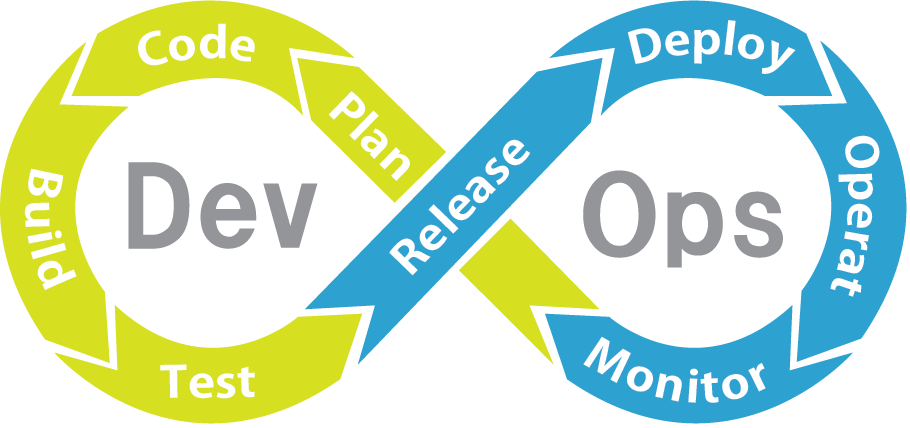
\includegraphics[width=\textwidth]{pic/general_workflow.png}
		\caption{Cloud DevOps provider}
	\end{subfigure}
\end{figure}  
DevOps is a kind of workflow management method in software engineering.
\end{frame}

\begin{frame}
\frametitle{Challenges in Experiment Reproducibility}

A given Python script from a Nature article gave different results on different Operating Systems [1]

\begin{itemize}
\item No source code
\item specific hardware requirement
\item specific software requirement
\item complex workflow, not clear to others
\end{itemize}

\vskip 1cm
{\tiny [1] J.~Bhandari~Neupane, R.~P. Neupane, Y.~Luo, W.~Y. Yoshida, R.~Sun, and P.~G.
  Williams, ``Characterization of leptazolines a--d, polar oxazolines from the
  cyanobacterium leptolyngbya sp., reveals a glitch with the
  “willoughby--hoye” scripts for calculating nmr chemical shifts,''
  \emph{Organic Letters}, 2019.
 } 
 
\end{frame}

\begin{frame}
\frametitle{Existing Method -- Specific Software Tools}

\begin{figure}
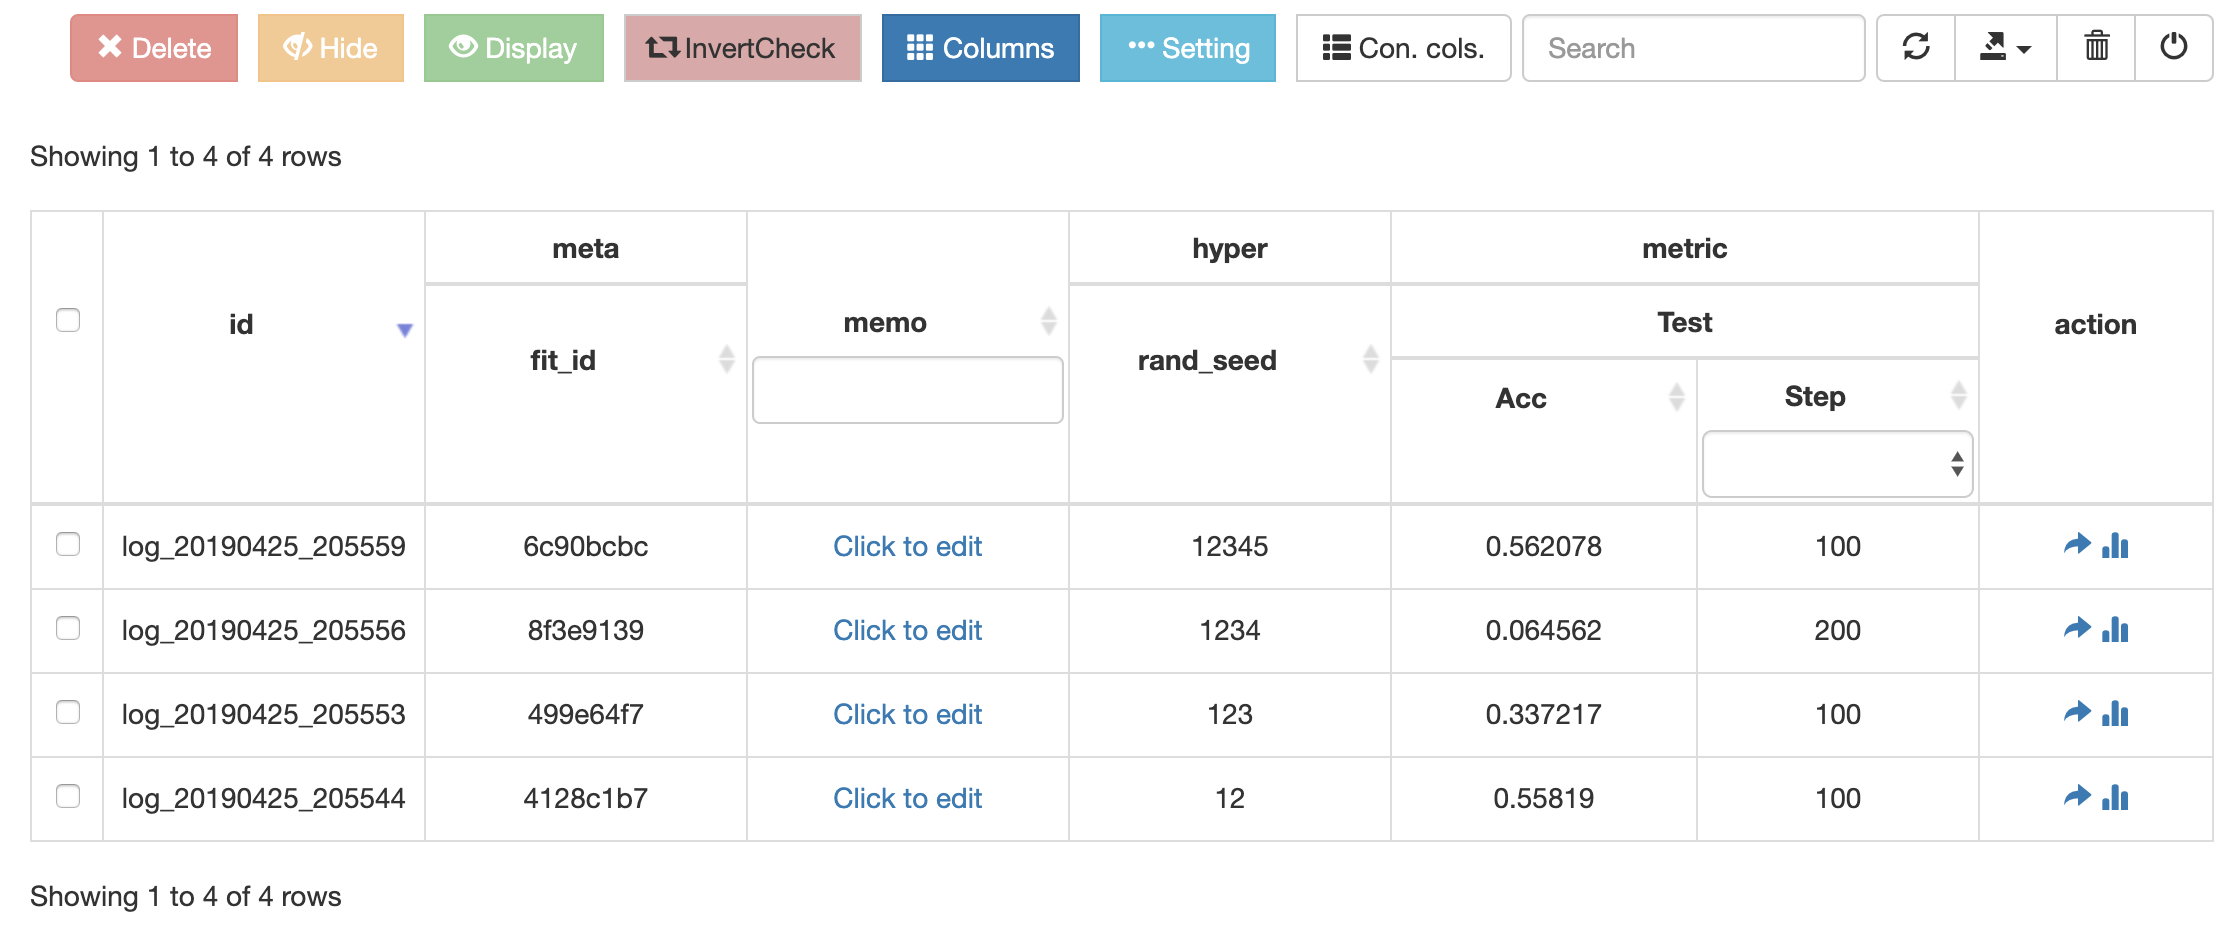
\includegraphics[width=0.8\textwidth]{pic/fitlog_table.png}
\caption{figlog package by FaskNLP Lab of FuDan University}
\end{figure}
Pros: running environment capture and experiment results storage

Cons: bad maintainability and difficult configuration
\end{frame}

\begin{frame}
\frametitle{Existing Method -- Out-of-box Platforms}

\begin{figure}
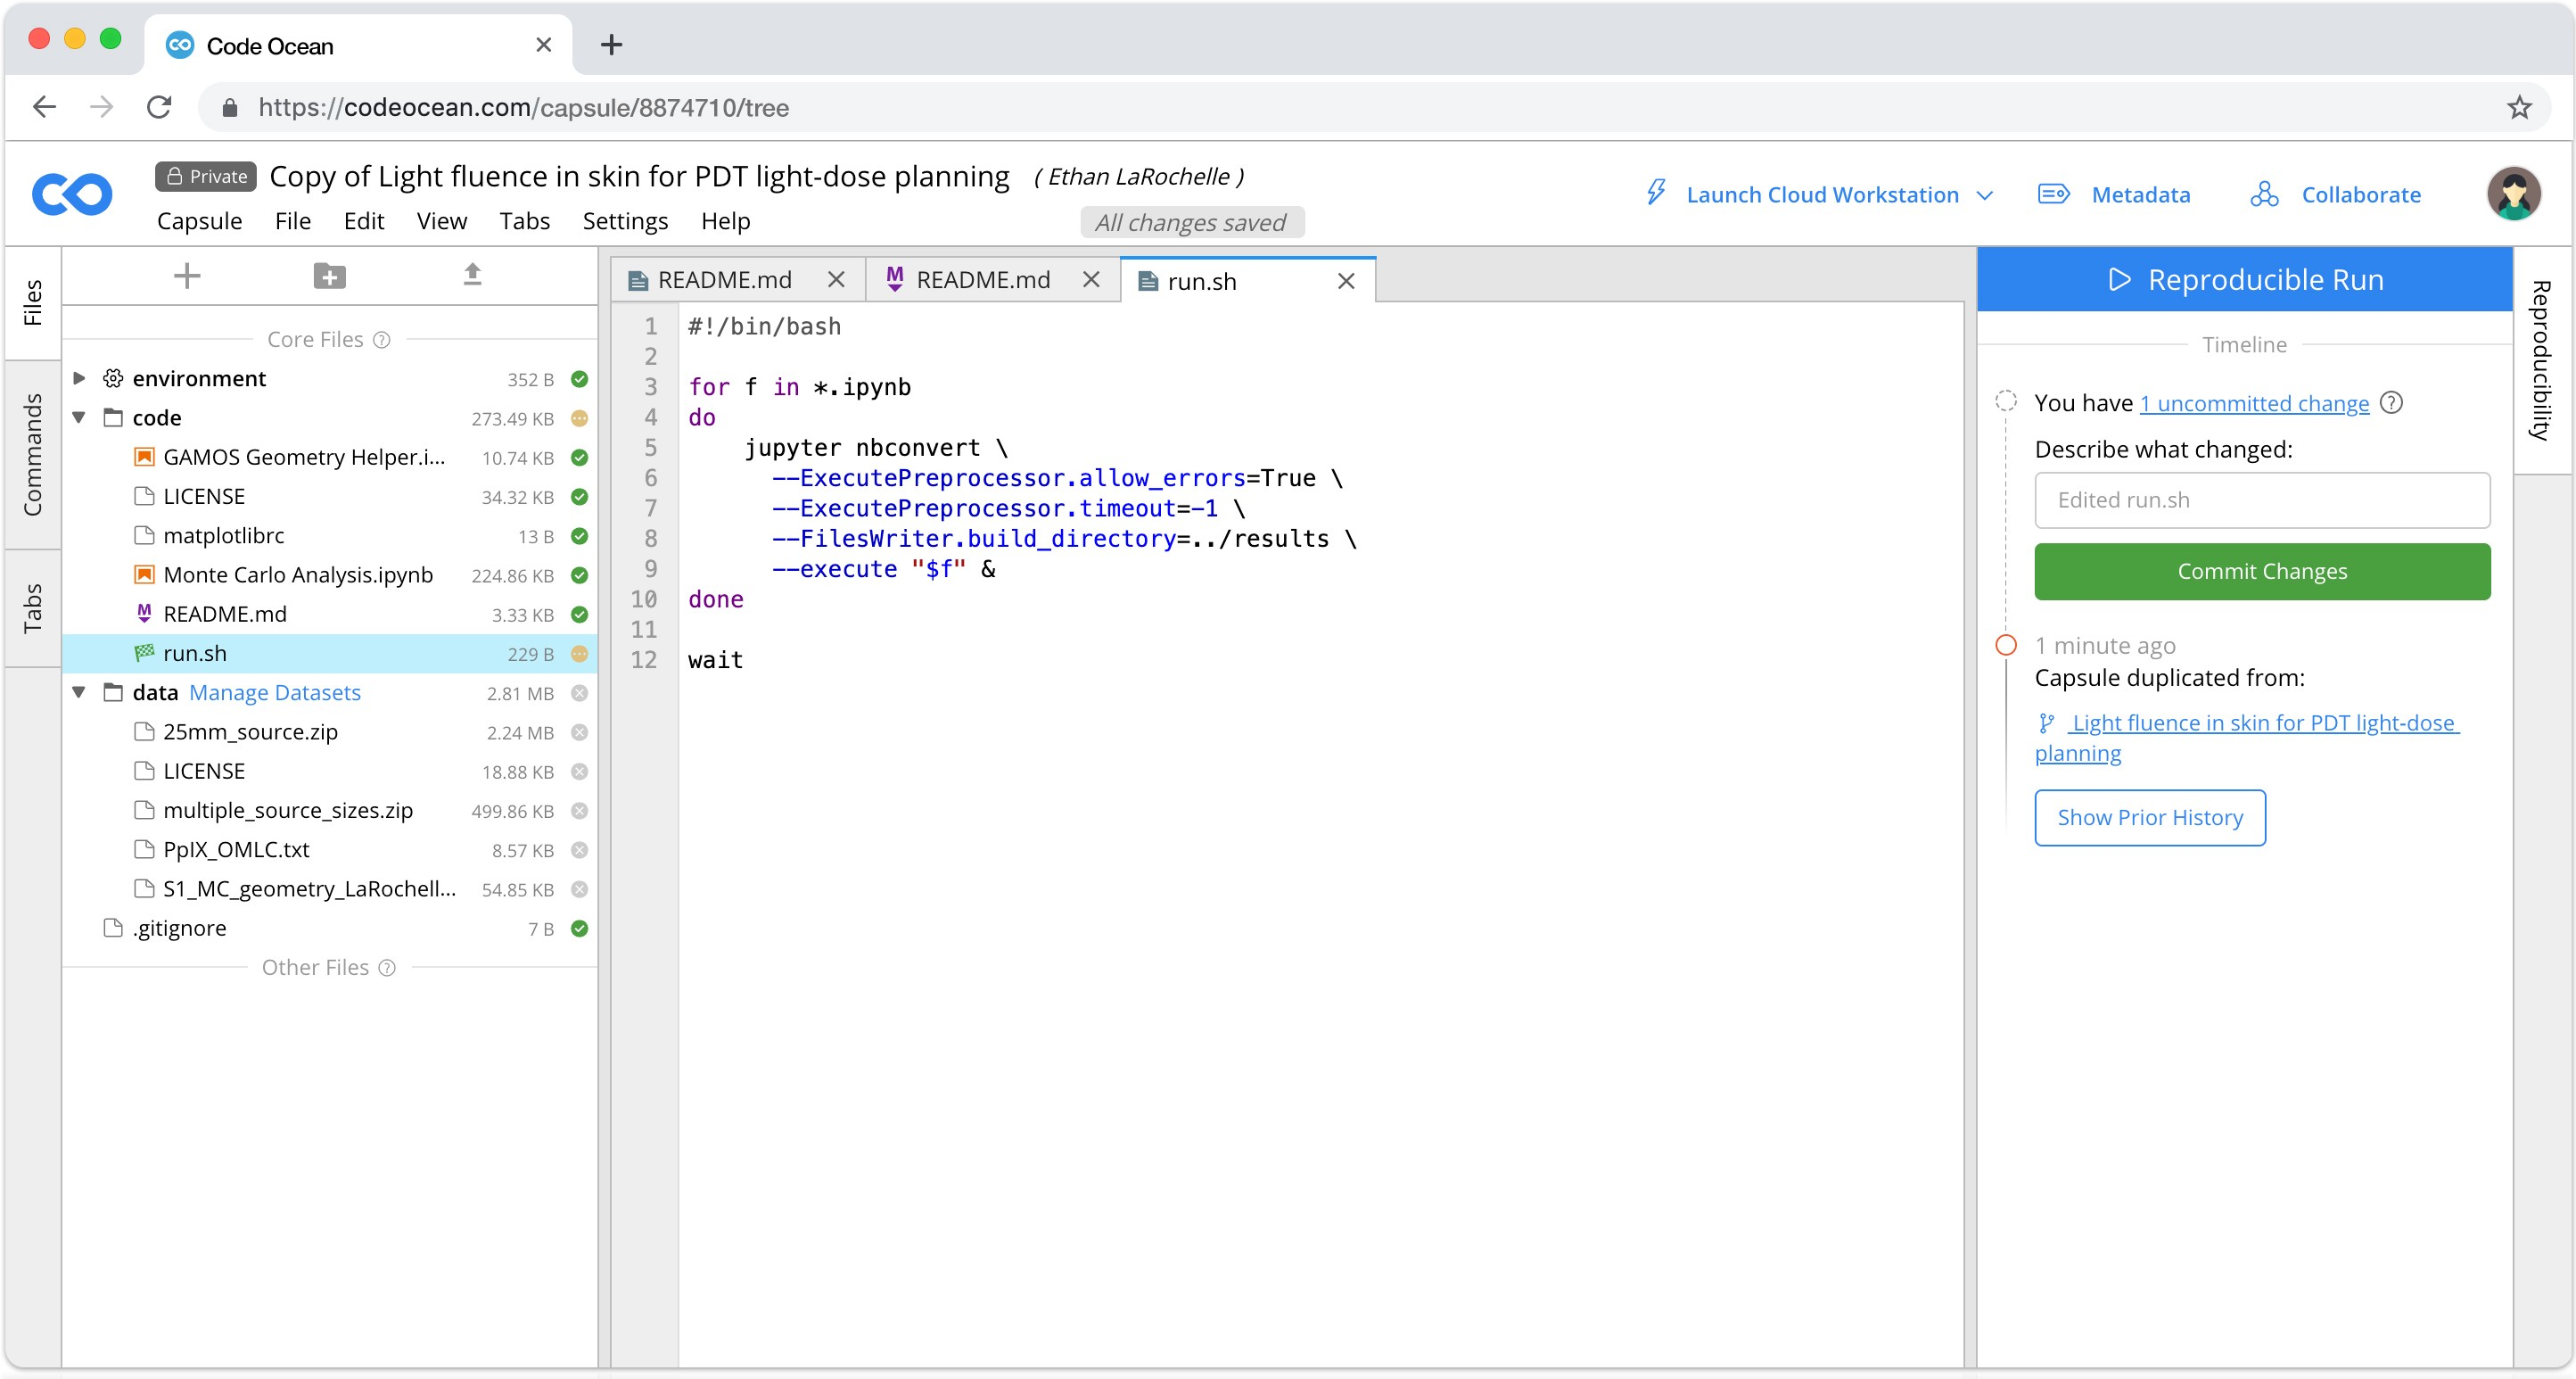
\includegraphics[width=0.8\textwidth]{pic/code_ocean.jpeg}
\caption{IEEE promoted codeocean platform}
\end{figure}
Pros: Uniform platform and easy to use

Cons: pay for your usage
\end{frame}

\begin{frame}
\frametitle{Existing Method -- Make Documentation}

\begin{itemize}
\item environment, software, external dataset etc.
\item documentation of each steps
\end{itemize}

Pros: no external barrier

Cons: varies between researchers
\end{frame}

\begin{frame}
\frametitle{Our Method -- Experiments with Cloud DevOps}
Advantages:
\begin{itemize}
	\item High availability of the service and well maintenance of the infrastructure
	\item Easy to use and flexible to configure
	\item Unlimited usage and rich computing resource
\end{itemize}
\end{frame}
\frame{\tableofcontents[currentsection]}
\section{Infrastructure}
\begin{frame}
\frametitle{What is DevOps}

Process of DevOps
\begin{figure}
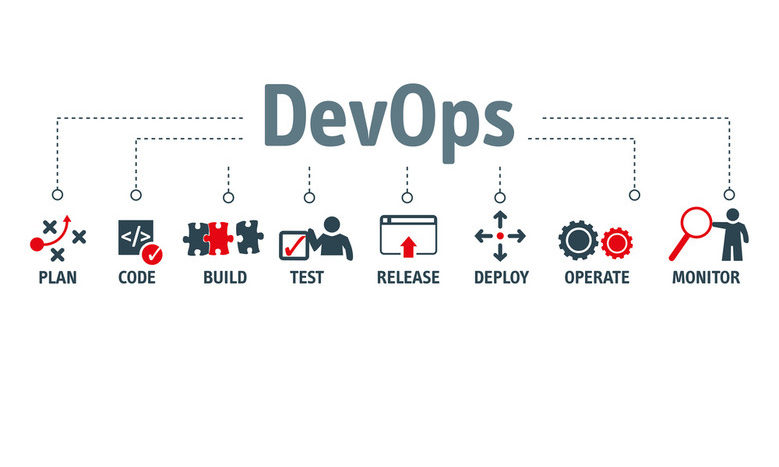
\includegraphics[width=5cm]{pic/what-is-devops.jpg}
\end{figure}
Core Components: Build and Deployment (CICD)
\end{frame}

\begin{frame}
\frametitle{Cloud DevOps service provider}

\begin{table}
\caption{Comparison of Cloud DevOps provider (until 2020)}
\label{table}
\small
\begin{tabular}{|@{\hspace{0.1em}}m{0.9cm}|@{\hspace{0.1em}}>{\centering}m{0.9cm}@{\hspace{0.9em}}|@{	\hspace{-0.1em}}>{\centering}m{0.9cm}|@{\hspace{0.2em}}>{\centering}m{0.8cm}|>{\centering}m{0.8cm}|>{\centering}m{1.0cm}|c|}
\hline
& 
{\scriptsize AppVeyor }& 
 {\scriptsize Azure pipelines} & {\scriptsize CircleCI } &  {\scriptsize GitLab CICD} & {\scriptsize GitHub Action}  & {\scriptsize Travis} \\
\hline
 {\scriptsize Platform} & {\scriptsize Windows Linux} & All & All & Linux docker & All & All\\
\hline
 {\scriptsize Parallel} & 1 & 10 & 4 & 8 &  20 & 5\\
 \hline
 {\scriptsize  Selfhost } & Y & Y & N & Y & Y & N\\
 \hline
 {\scriptsize Artifact} & N & Y & Y & Y & Y & N\\
 \hline
\end{tabular}
\label{tab1}
\end{table}
\end{frame}

\begin{frame}[fragile]
\frametitle{Choosing Environment for Agent}
\begin{enumerate}
\item virtual machine or docker container.
\item public cloud service or local runner.
\item programming language and version.
\end{enumerate}

\begin{lstlisting}[caption={environment configuration}, captionpos=b]
os: linux
dist: xenial
language: python
python: 3.6
\end{lstlisting}
\end{frame}

\begin{frame}[fragile]
\frametitle{Workflow Principle}
\begin{figure}
\centering
\begin{subfigure}{0.4\textwidth}
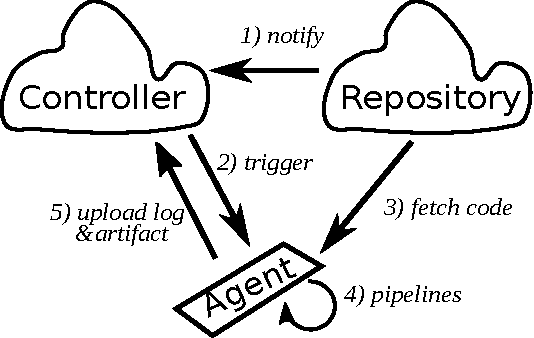
\includegraphics[width=\textwidth]{../principal.pdf}
\caption{Interaction of different components}
\end{subfigure}~
\begin{subfigure}{0.4\textwidth}
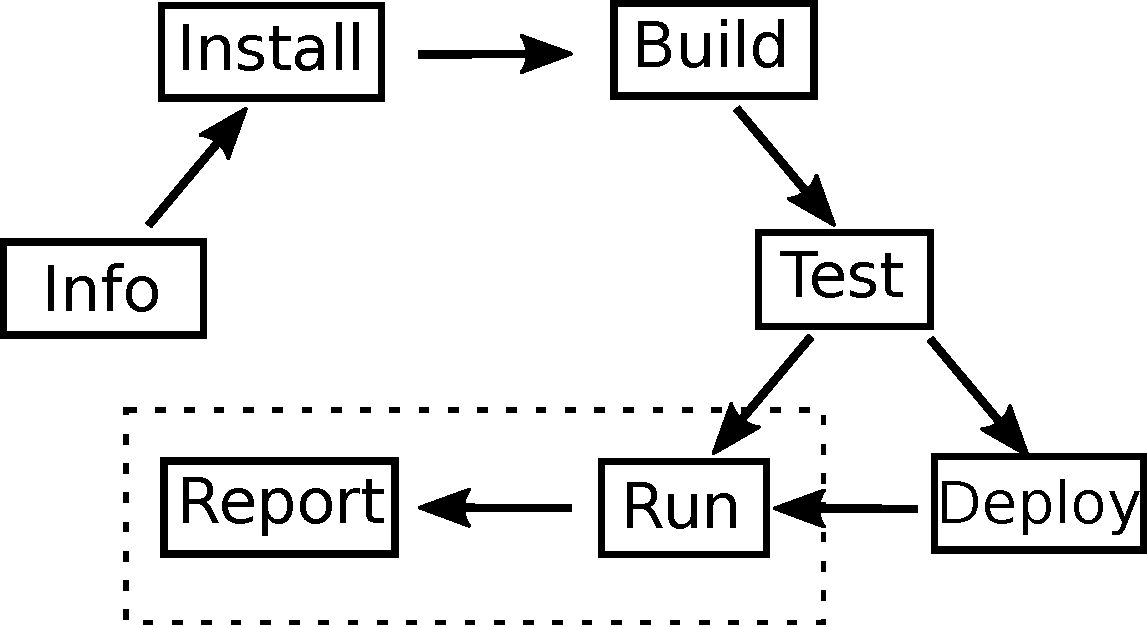
\includegraphics[width=\textwidth]{../workflow.pdf}
\caption{pipelines for scientific experiments}
\end{subfigure}
\end{figure}

\begin{lstlisting}[caption={workflow description}, label={lst:wd}, captionpos=b]
install: 
  - pip install -r requirements.txt
script: # run experiment
  - python main.py
\end{lstlisting}

\end{frame}
\frame{\tableofcontents[currentsection]}
\section{Case Studies}
\begin{frame}
\frametitle{Using public agent}
\begin{itemize}
\item implementating a triangle counting algorithm in C++
\item deploy the package to Ubuntu PPA
\item run the medium-scale experiment on Travis CI public server
\end{itemize}
Server VM has 2 CPU cores and 7.5 GB memory space.

Our program finishes in 4.3 minutes and consumes 3.1GB memory.
\end{frame}
\begin{frame}
\frametitle{Using self-hosted agent}
\begin{itemize}
\item Using OpenMP to parallel the triangle counting algorithms
\item the experiment is run using a computing node with 32 CPUs.
\item the running log is uploaded to server automatically.
\end{itemize}
\begin{figure}
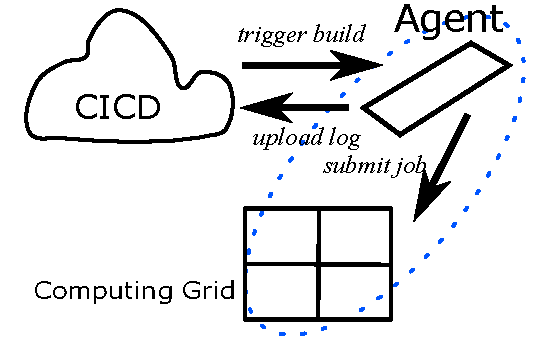
\includegraphics[width=5cm]{../self-hosted.pdf}
\caption{self-hosted computing cluster connected to DevOps server}
\end{figure}
\end{frame}

\begin{frame}
\frametitle{incorporating other cloud infrastructure}
\begin{itemize}
\item incorporate a serverless computing experiment
\item replace the private client with public agent
\end{itemize}
\begin{figure}
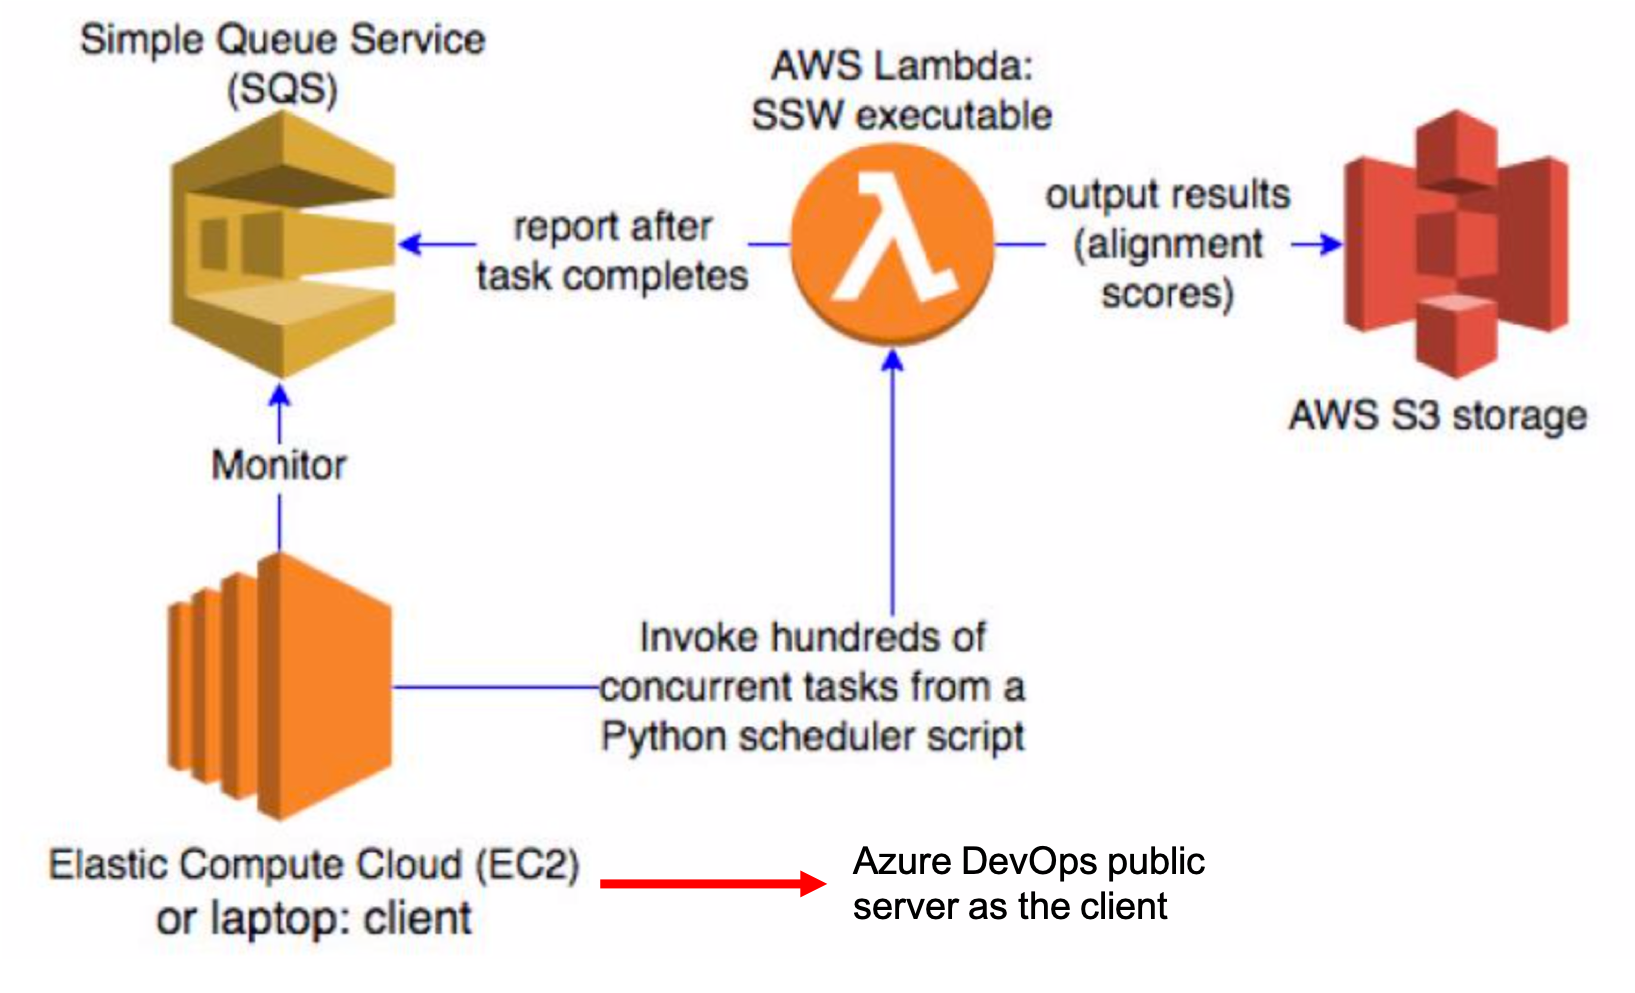
\includegraphics[width=0.8\textwidth]{pic/serverless_show.png}
\end{figure}
\end{frame}
\section{Conclusion}
\begin{frame}
\frametitle{Conclusion}
\begin{itemize}
\item Researchers should make their experiments reproducible
\item Cloud DevOps is a good chice for such purpose
\end{itemize}
\end{frame}

\begin{frame}
\frametitle{}
\begin{block}{}
\centering
{\Huge Thank you!}
\end{block}
\end{frame}
\end{document}
